\levelstay{Parallel LC}

Before studying true qubits, we consider a parallel LC circuit as shown in Fig.\,\ref{Fig:singleCircuit}.
Although this circuit is harmonic and therefore impractical to use as a qubit, it is explicitly solvable and provides a good intuition about the dependence of important parameters such as coupling strength on qubit properties such as impedance and frequency.
Moreover, for weakly anharmonic qubits like the transmon, we can find good approximations by starting with harmonic oscillator analysis and then subsituting
\begin{equation*}
  a + a^\dagger \rightarrow \sigma_x
  \quad \textrm{and} \quad
  a - a^\dagger \rightarrow i \sigma_y \, .
\end{equation*}

From Kirchhoff's laws, one can derive the equations of motion for the flux through the LC oscillator's inductor:
\begin{equation*}
  \ddot{\Phi} + \omega_{LC}^2 \Phi = 0
\end{equation*}
where $\omega_{LC}=1/\sqrt{LC}$.
This equation of motion is reproduced by the Lagrangian \footnote{Lagrange's equation of motion is $\frac{d}{dt}\left( \frac{\partial L}{\partial \dot{\Phi}} \right) - \frac{\partial L}{\partial \Phi} = 0$.}
\begin{equation*}
  \mathcal{L} = \frac{1}{2}C\dot{\Phi}^2 - \frac{1}{2L}\Phi^2
\end{equation*}
The momentum conjugate to the flux $\Phi$ is, by definition,
\begin{equation*}
  \text{momentum} \equiv \frac{\partial \mathcal{L}}{\partial \dot{\Phi}} = C\dot{\Phi} = Q \, .
\end{equation*}
We denote the canonical momentum as $Q$ because $\dot{\Phi}$ is the voltage across the LC circuit (remember that inductance is defined by $V = L \dot{I} = \dot{\Phi}$), so $C \dot{\Phi} = Q$ is the charge on the capacitor.
Therefore, $\Phi$ and $Q$ are so-called canonically conjugate variables.

The Hamiltonian is, again by definition,
\begin{equation}
  H
  = \frac{\partial \mathcal{L}}{\partial \dot{\Phi}} \dot{\Phi} - \mathcal{L}
  = \frac{Q^2}{2C} + \frac{\Phi^2}{2L} \, . \label{eq:shoHamiltonian}
\end{equation}
The analysis so far has been entirely classical, but if the circuit is sufficiently decoupled from noisy environmental degrees of freedom, it behaves quantum mechanically and we should think of $\Phi$ and $Q$ as operators!
As these operators are canonically conjugate, we have (either by postulates of quantum mechanics or by practical experience) $[\Phi,Q]=i\hbar$.
Equation (\ref{eq:shoHamiltonian}) and the commutation relation provide the complete starting point for the study of the LC oscillator in quantum mechanics.
The quantum harmonic oscillator is studied in \citeinternaltype \citeinternalref{quantumOscillator} where it is found that the Hamiltonian can be re-expressed as
\begin{align}
  \frac{H}{\hbar \omega_{LC}}
  &= \left( \frac{1}{2} + a^\dagger a \right) \nonumber \\
  &= \frac{\varphi^2}{2} \left( \frac{R_K / 8 \pi}{Z_{LC}} \right)
   + \frac{n^2}{2} \left( \frac{Z_{LC}}{R_K / 8 \pi} \right)
\end{align}
where
\begin{align}
  \varphi &\equiv 2 \pi \Phi / \Phi_0 \, , \quad n \equiv Q / 2e \, , \quad [\varphi, n] = i \\
  a &\equiv
      \frac{1}{2} \frac{\Phi}{\Phi_\text{zpf}}
  + i \frac{1}{2} \frac{Q}{Q_\text{zpf}} \\
  \Phi_\text{zpf} &\equiv \sqrt{\frac{\hbar Z_{LC}}{2}} \, , \quad
  Q_\text{zpf} \equiv \sqrt{\frac{\hbar}{2 Z_{LC}}}
\end{align}
and
\begin{equation}
  Z_{LC} \equiv \sqrt{L/C} \, .
\end{equation}

\begin{figure}
\begin{centering}
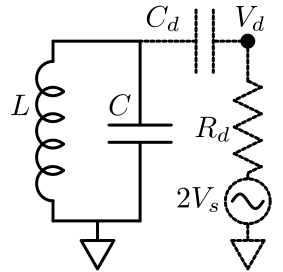
\includegraphics[width=4cm]{single_circuit_with_drive.pdf} 
\par\end{centering}
  \caption{A parallel LC circuit with capacitively coupled driving. The main circuit is shown in solid line, while the driving circuit is shown in dotted line.}
\label{Fig:singleCircuit}
\end{figure}

